% !Mode:: "TeX:UTF-8"
\documentclass{article}
\usepackage[hyperref, UTF8]{ctex}
\usepackage[dvipsnames]{xcolor}
\usepackage{geometry}
\usepackage{amsmath}
\usepackage{amsfonts}
\usepackage{listings}
\usepackage{pgfplotstable}
\usepackage{pgfplots}
\usepackage{fontspec}
\usepackage{booktabs} % 表格上的不同横线
%\setmainfont{Consolas} %设置英文字体

\definecolor{mygreen}{rgb}{0,0.6,0}
\definecolor{mygray}{rgb}{0.5,0.5,0.5}
\definecolor{mymauve}{rgb}{0.58,0,0.82}
\lstset{ %
    backgroundcolor=\color{white},   % choose the background color
    basicstyle=\footnotesize\ttfamily,        % size of fonts used for the code
    columns=fullflexible,
    breaklines=true,                 % automatic line breaking only at whitespace
    captionpos=b,                    % sets the caption-position to bottom
    tabsize=4,
    backgroundcolor=\color[RGB]{245,245,244},            % 设定背景颜色
    commentstyle=\color{mygreen},    % comment style
    escapeinside={\%*}{*)},          % if you want to add LaTeX within your code
    keywordstyle=\color{blue},       % keyword style
    stringstyle=\color{mymauve}\ttfamily,     % string literal style
    showstringspaces=false,                % 不显示字符串中的空格
    frame=none,
    rulesepcolor=\color{red!20!green!20!blue!20},
    % identifierstyle=\color{red},
    language=c++,
}

% 设置hyperlink的颜色
\newcommand\myshade{85}
\colorlet{mylinkcolor}{violet}
\colorlet{mycitecolor}{YellowOrange}
\colorlet{myurlcolor}{Aquamarine}


\title{系统/子系统设计(结构设计)说明(后台部分)}
\author{Tomato}
\date{2018年1月}

\begin{document}

    \maketitle
        \section{引言}
            \subsection{系统概述}
                后台分为两个部分,上层是Controller,是用来处理业务逻辑的,下层是数据库,给上层的Controller提供相应的服务。下面会分两块来具体介绍这两部分。详见《接口设计说明》和《数据库(顶层)设计说明》。

            \subsection{文档概述}
                本文档将围绕Spring Boot架构来介绍后台部分。
        \section{系统级设计决策}
            本系统后台主要使用Spring Boot架构,它支持在开启服务的时候,接受HttpRequest或websocket并进行后台处理,然后返回相应的结果。系统接受的输入是HttpRequest或websocket,详见《接口设计说明》,对于每一个输入的响应,被Controller定义,不同的request会有不同的Controller对其进行处理并返回相应的结果。系统处理的过程中,依赖于两部分的内容:用户的request中的具体内容和底层数据库已有的信息。详见《数据库(顶层{设计说明}》。该系统的数据库存在服务器上,服务器的管理人员可以通过database asdan来访问数据库并查看当前数据库中的所有信息。该系统对服务器的要求是要求服务器能通过maven运行项目,并配有mysql数据库。
        \section{系统体系结构设计}
            \subsection{系统总体设计}
                \paragraph{概述}
                    本系统要实现的功能详见《prj9ASDAN模拟商业竞拍交易大赛系统》。本系统要实现的性能:响应较快、支持并发、有一定的安全性、可在各个平台上运行、可移植等。本系统支持在Windows、Unix、Linux环境下运行。
                \paragraph{设计思想}
                    本系统顶层核心要处理的两个问题是对于HttpRequest的处理和对于websocket的处理,而底层核心要处理的问题是数据库的维护等问题。如果直接从头开始开发一套框架,则要实现的内容可能比我们当前写的多得多。所以我们后台根据这个需求找到了Spring Boot框架。Spring Boot 很好地通过了Annotations来实现我们需要的对于前端web端的响应,也实现了我们需要的和数据库的连接、并发的响应等等。本系统并不需要很高深的算法,但是对逻辑上的要求十分的多和细致。
                \paragraph{基本处理流程}
                    下面以用户登录为例来讲解后台对于HttpRequest的处理流程。

                    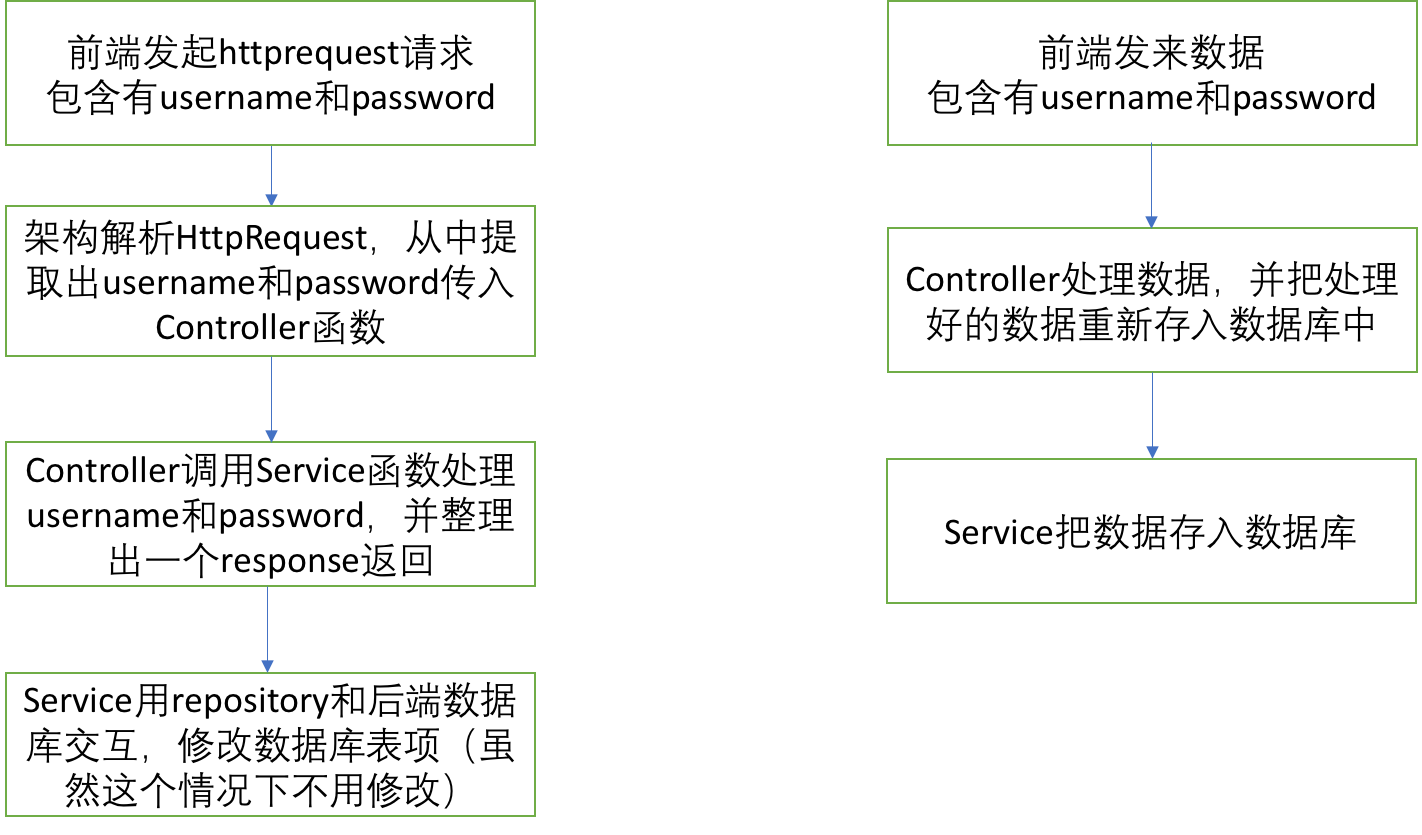
\includegraphics[scale = .3]{fig/基本数据.png}

                    当前端发来HttpRequest或websocket的时候,Controller首先会提取出发来的数据内容,然后将根据业务逻辑处理数据,在处理数据的过程中,可能需要访问数据库中已有的数据,如在这个情况下需要对拍数据库中的账号和密码。也有可能需要修改后台数据库,但是图中的例子不需要。在处理完数据之后,Controller会把数据重新包装,然后根据API文档的说明传回前端。整个数据处理的过程可以理解为从前端发来数据,然后Controller向数据库query数据,然后处理完数据之后又save到数据库中,最后返回给前端。
                \paragraph{系统体系结构}
                    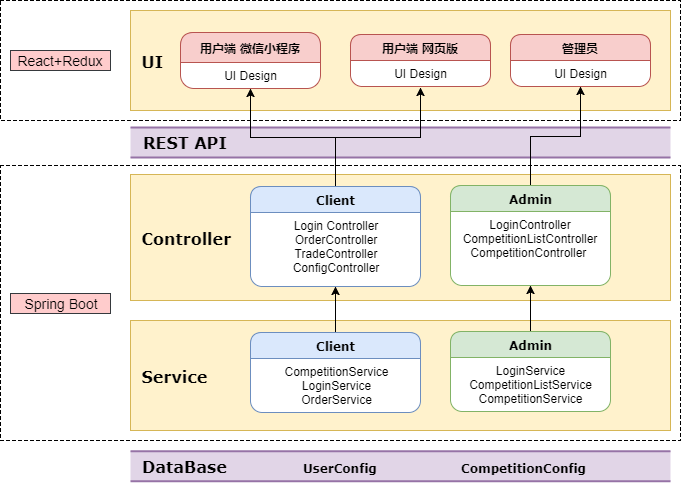
\includegraphics[scale = .3]{fig/架构图.png}

                    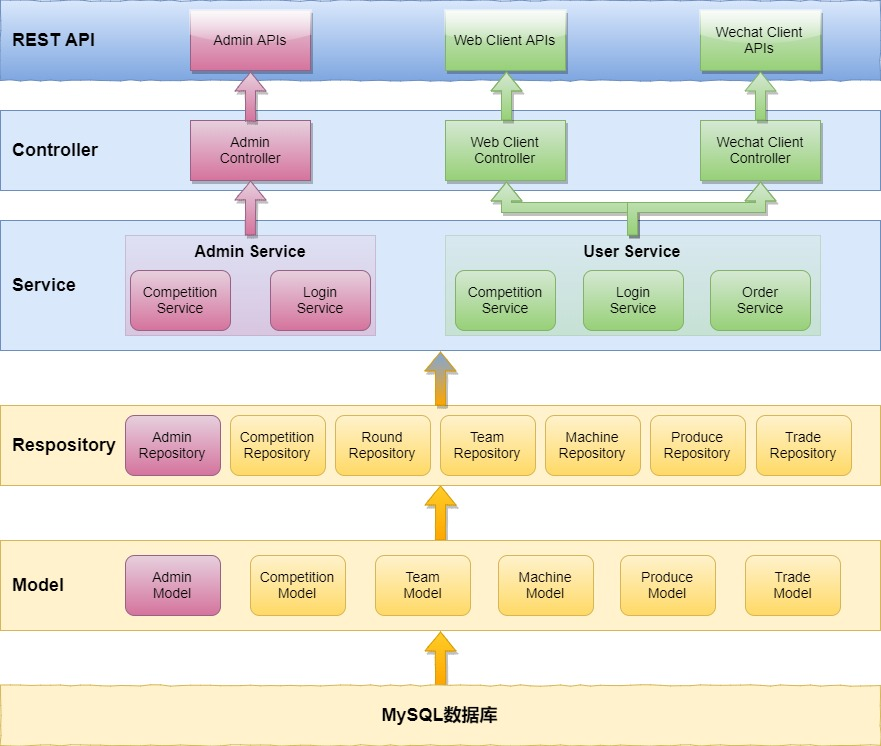
\includegraphics[scale = .3]{fig/有用.jpeg}

                    如图,前端的功能是响应用户的操作,并把用户操作的数据根据API文档中的要求进行包装,作为HttpRequest或websocket发往后端,后端Controller对于包装好的数据解码,并query Service,和数据库交互,完成数据的处理,并完成数据库的更新。最后将HttpRequest返回给前端或将websocket转发。
            \subsection{接口设计}
                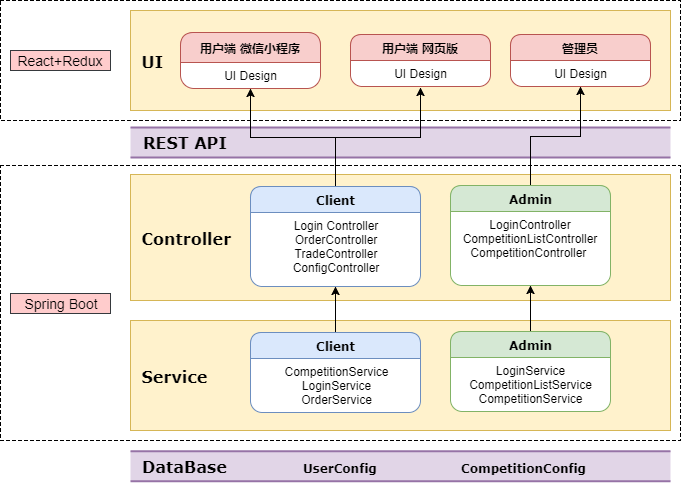
\includegraphics[scale = .3]{fig/架构图.png}
        \section{系统出错处理设计}
            系统出错后,后台数据库的内容不会被清空,并且我们是在处理request流程中对数据库是实时更新的,宕机之后数据库的内容还是会保留,当下次启动服务器的时候它还能从原数据库中获得原来的数据,并根据这些数据进行处理。

            当系统出错后,建议重启服务器。
        \section{尚待解决的问题}
            微信后端的websocket的测试问题。

\end{document}
